\documentclass[titlepage,numbers=noenddot,headinclude,%1headlines,% letterpaper a4paper
                footinclude=false,cleardoublepage=empty,
                BCOR=5mm,paper=a4,fontsize=11pt,11pt,a4paper,american
                ]{scrreprt}
                \usepackage[english]{babel}
\newcommand{\bflabel}{\aclabelfont}

%********************************************************************
% Note: Make all your adjustments in here
%*******************************************************
\input{classicthesis-config}

%********************************************************************
% Hyphenation
%*******************************************************
%\hyphenation{put special hyphenation here}

% ********************************************************************
% GO!GO!GO! MOVE IT!
%*******************************************************
\begin{document}
\frenchspacing
\raggedbottom
%\renewcommand*{\bibname}{new name}
%\setbibpreamble{}
\pagenumbering{roman}
\pagestyle{plain}
%********************************************************************
% Frontmatter
%*******************************************************
\thispagestyle{empty}
\begin{titlepage}
   \begin{addmargin}[-1cm]{-3cm} % requires KOMA class. Why do I need this fuckery?

      \vspace*{2cm}

      \begin{center}

         \Large

         
\includegraphics[width=.7\textwidth]{gfx/uni.pdf}

         \vspace{2cm}

         {
            \LARGE \emph{Bachelor's Thesis}
         }

         \vspace{2cm}

         {
            \Huge 
            \myTitle
         }

         \vspace{2cm}

         {
            \LARGE
            Rasmus Diederichsen
         }

         \vspace{2cm}

         {
            \begin{tabular}{>{\bfseries}ll}
               First Supervisor: & \myFirstSupervisor \\
               Second Supervisor: & \mySecondSupervisor
            \end{tabular}
         }

         \vspace{2cm}

         {
            Department of Computer Science

            Department of Cognitive Science
         }
      \end{center}
   \end{addmargin}
\end{titlepage}

\cleardoublepage\include{FrontBackmatter/Dedication}
\cleardoublepage\chapter*{Abstract}

Rephotography is the process of recreating a historic photograph by finding the
exact pose and ideally the exact camera parameters to then take a picture from
the same spot. The original and new images
can be used to document the passage of time and the changes which a static scene
has undergone, for instance by blending the two images together. Traditionally,
the exercise is carried out by photographers via careful examination of the
current camera picture and comparing it with the original image, gradually
moving the camera until an optimal registration is achieved. Besides being very
laborious, this approach is also quite error-prone, motivating the desire for
computerised assistance.

The ubiquity of camera-enabled mobile devices which---contrarily to
cameras---can be programmed allows such assistance to be provided, but few aids
are available. Two mobile applications simplify the procedure, yet still the
photographer is required to determine the necessary motion on their own. This
thesis presents an attempt to reproduce a more sophisticated system which was
prototyped for a laptop with connected camera as a mobile application. This
approach makes use of image processing in order to tell the user how to move the
camera to recover the original viewpoint.

The theoretical and practical challenges in computing a necessary motion are
explored and the system implemented as an iOS application. A detailed
evaluation of the results is performed, concluding that the reproduction was
partially successful, but some aspects of the pose recovery require further work.

\cleardoublepage\chapter*{Acknowledgments}

I wish to acknowledge the contributions of many people who---directly or
indirectly---supported this work. 

I thank Professor Oliver Vornberger, whose proposal of this topic came just at
the right time and who granted me the freedom to shape it on my own terms, and
Ann-Katrin Becker who drafted the initial plan for the application and
proved to be a constant source of useful advice.

Furthermore, I am grateful to Dr. Thomas Wiemann for his tech support
whenever CMake refused to bend to my will, and his readiness to act as
co-examiner.

None of the work would have been possible without the countless indviduals who
developed the long list of open source tools which I use on a daily basis.
Notably the entire \LaTeX\ community---developers and helpful users alike, the
developers of the OpenCV library, Vim, git and all UNIX tools and the
StackOverflow community where few questions go unanswered.

Writing a thesis is dull, especially alone and thus I was happy to suffer and
occasionally laugh alongside Inga, Lara and Lisa, who---perhaps unbeknownst to
them---kept my motivation on an at least partially productive level and Simon
and Julius for providing shelter and squirrels in times of need.

Particular thanks are owed to Lisa and Lea for proofreading this work.

% Lastly, I owe a great debt to my family whose support knows no bounds. For this,
% there are no words, so I shall give none.

\pagestyle{scrheadings}
\cleardoublepage\include{FrontBackmatter/Contents}
%********************************************************************
% Mainmatter
%*******************************************************
\pagenumbering{arabic}
%\setcounter{page}{90}
% use \cleardoublepage here to avoid problems with pdfbookmark
\cleardoublepage
\chapter{Introduction}
Rephotography denotes the retrieval of the precise viewpoint used for taking a
--- possibly historic --- photograph and capturing another image from the same
spot, ideally with the same camera parameters. This allows for
documentation and visualisation of changes which the scene has undergone between
the two or more captures.  For instance, one can present progress of
construction, restoration efforts or changes in the surroundings in a visually
striking manner, for instance by blending the photographs together. 
Figures \autoref{fig1} and \autoref{fig2} show examples.

\begin{figure}
   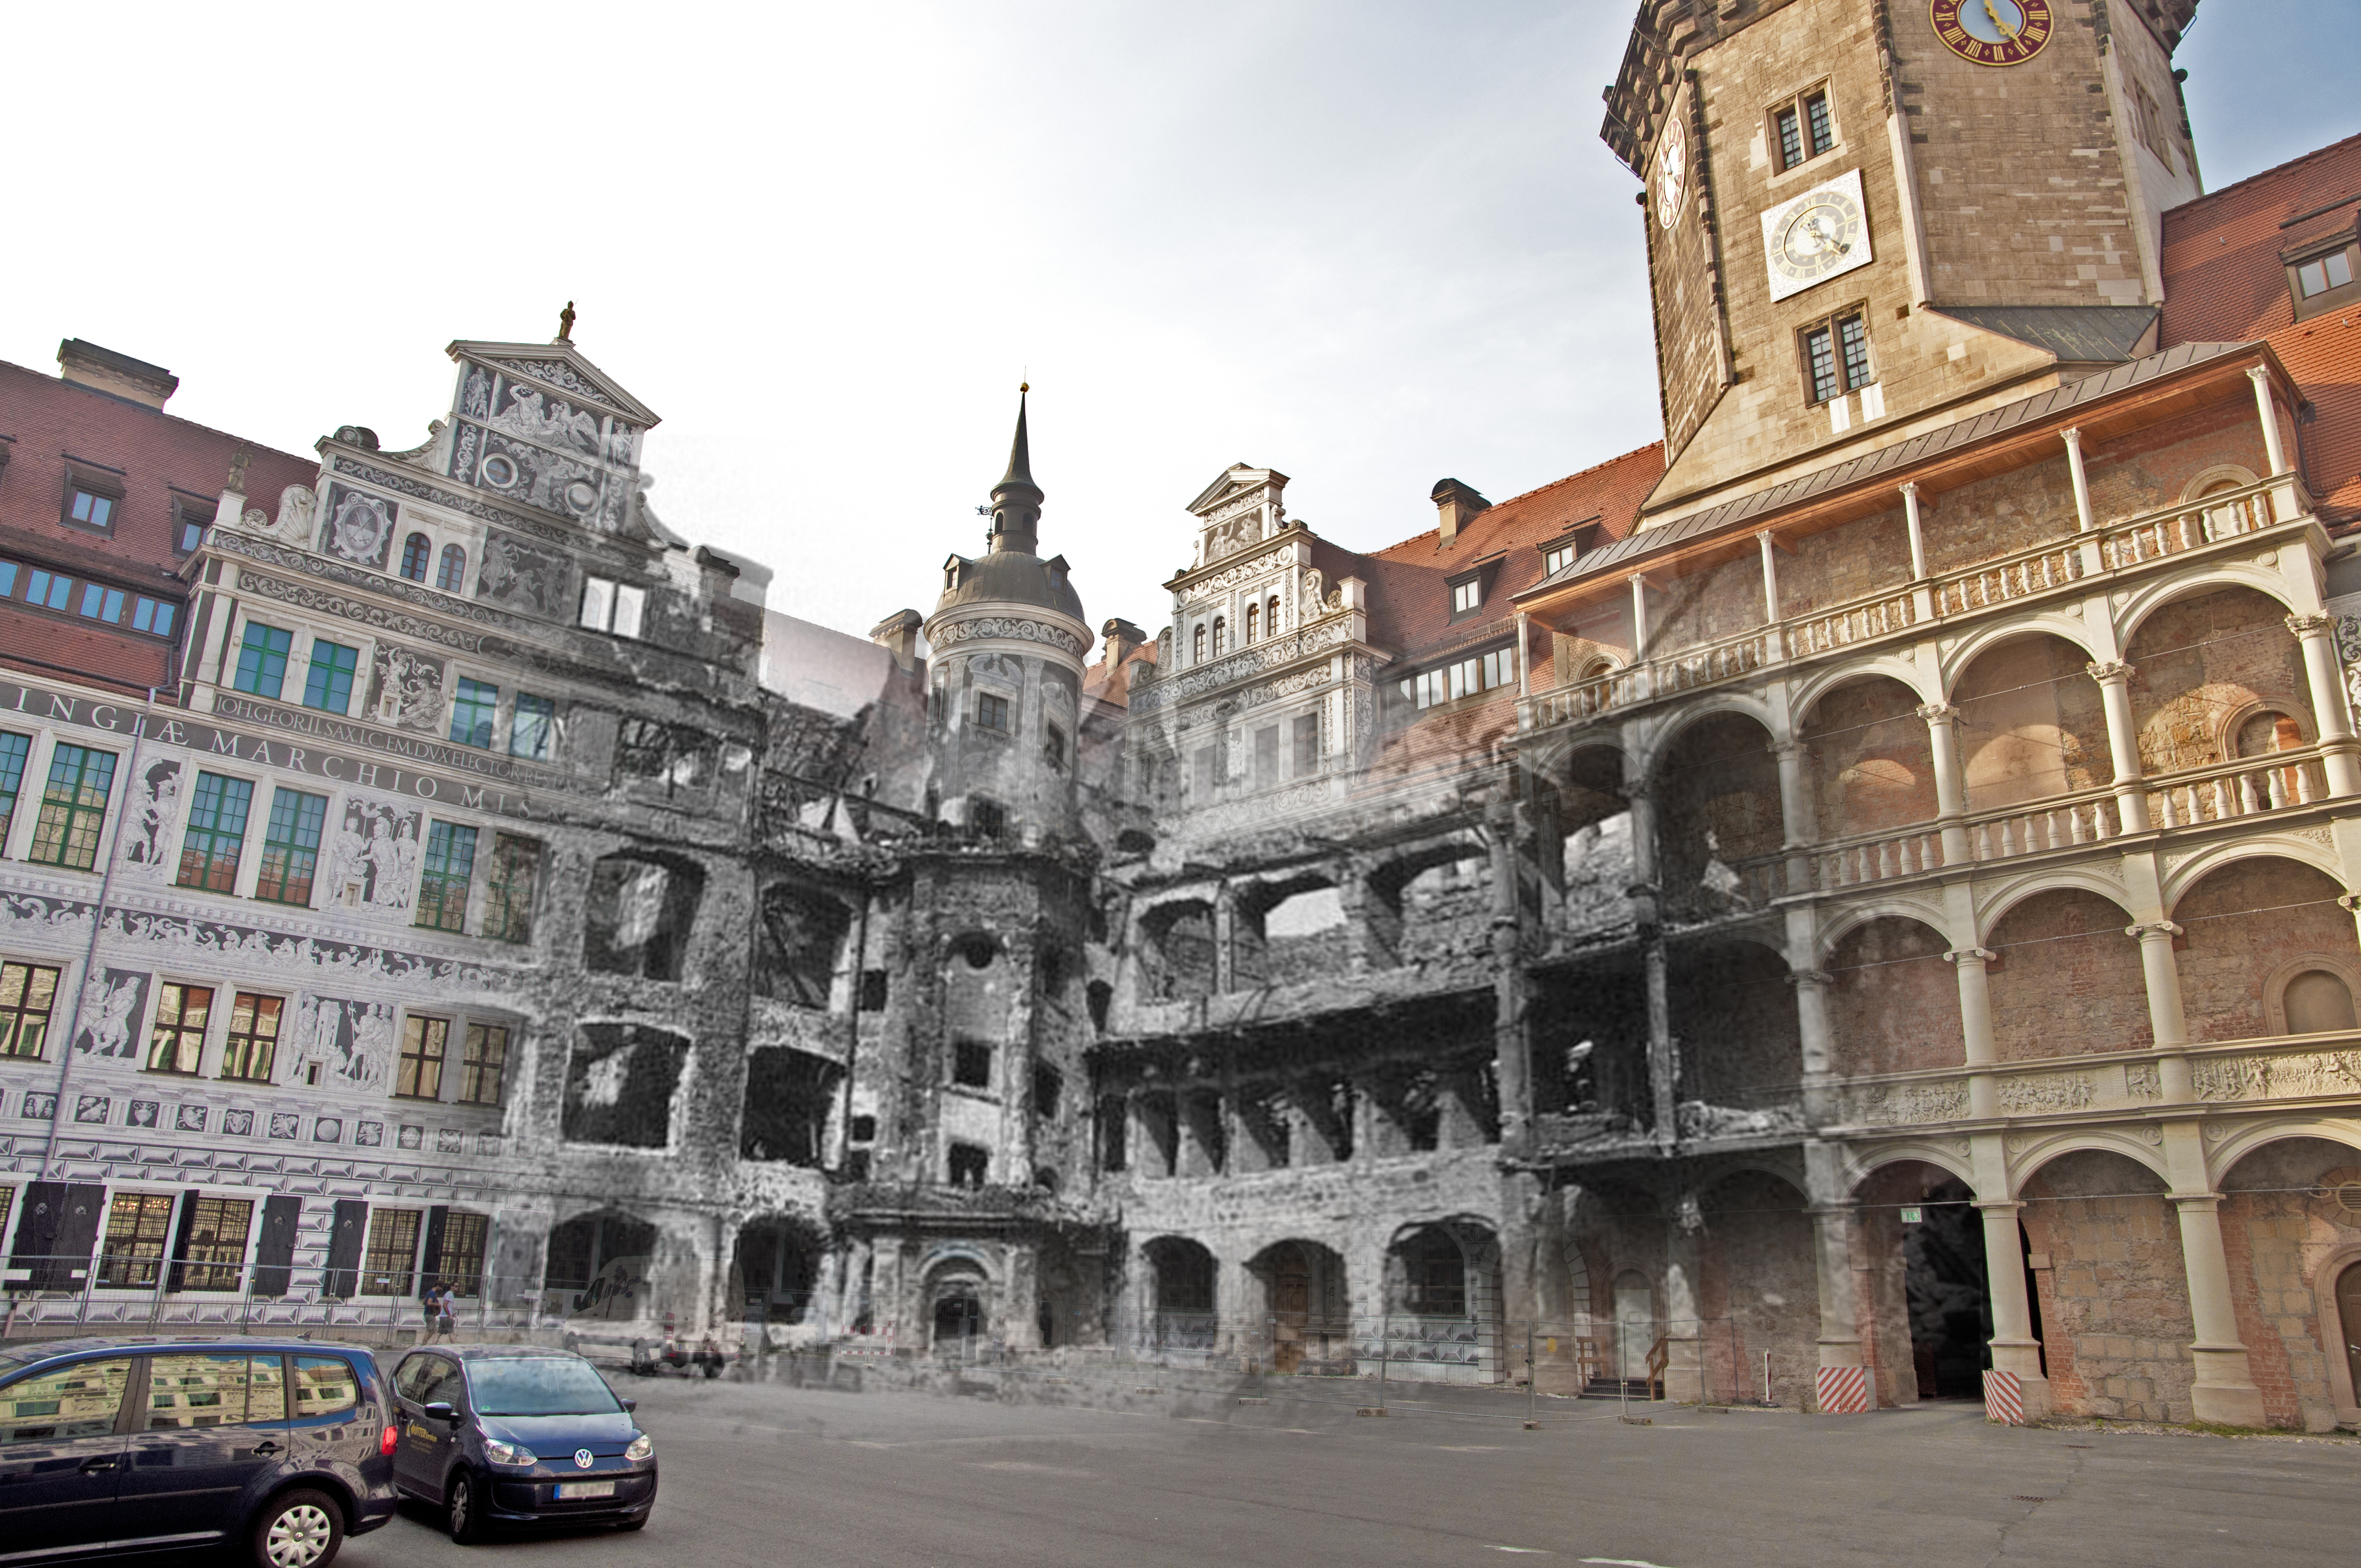
\includegraphics[width=\textwidth]{gfx/1945_2014_Residenzschloss.jpg}
   \caption{Residenzschloss in Dresden, destroyed during World War II,
   \textcopyright\ Sergey Larenkov, printed with permission}
   \label{fig1}
\end{figure}

\begin{figure}
   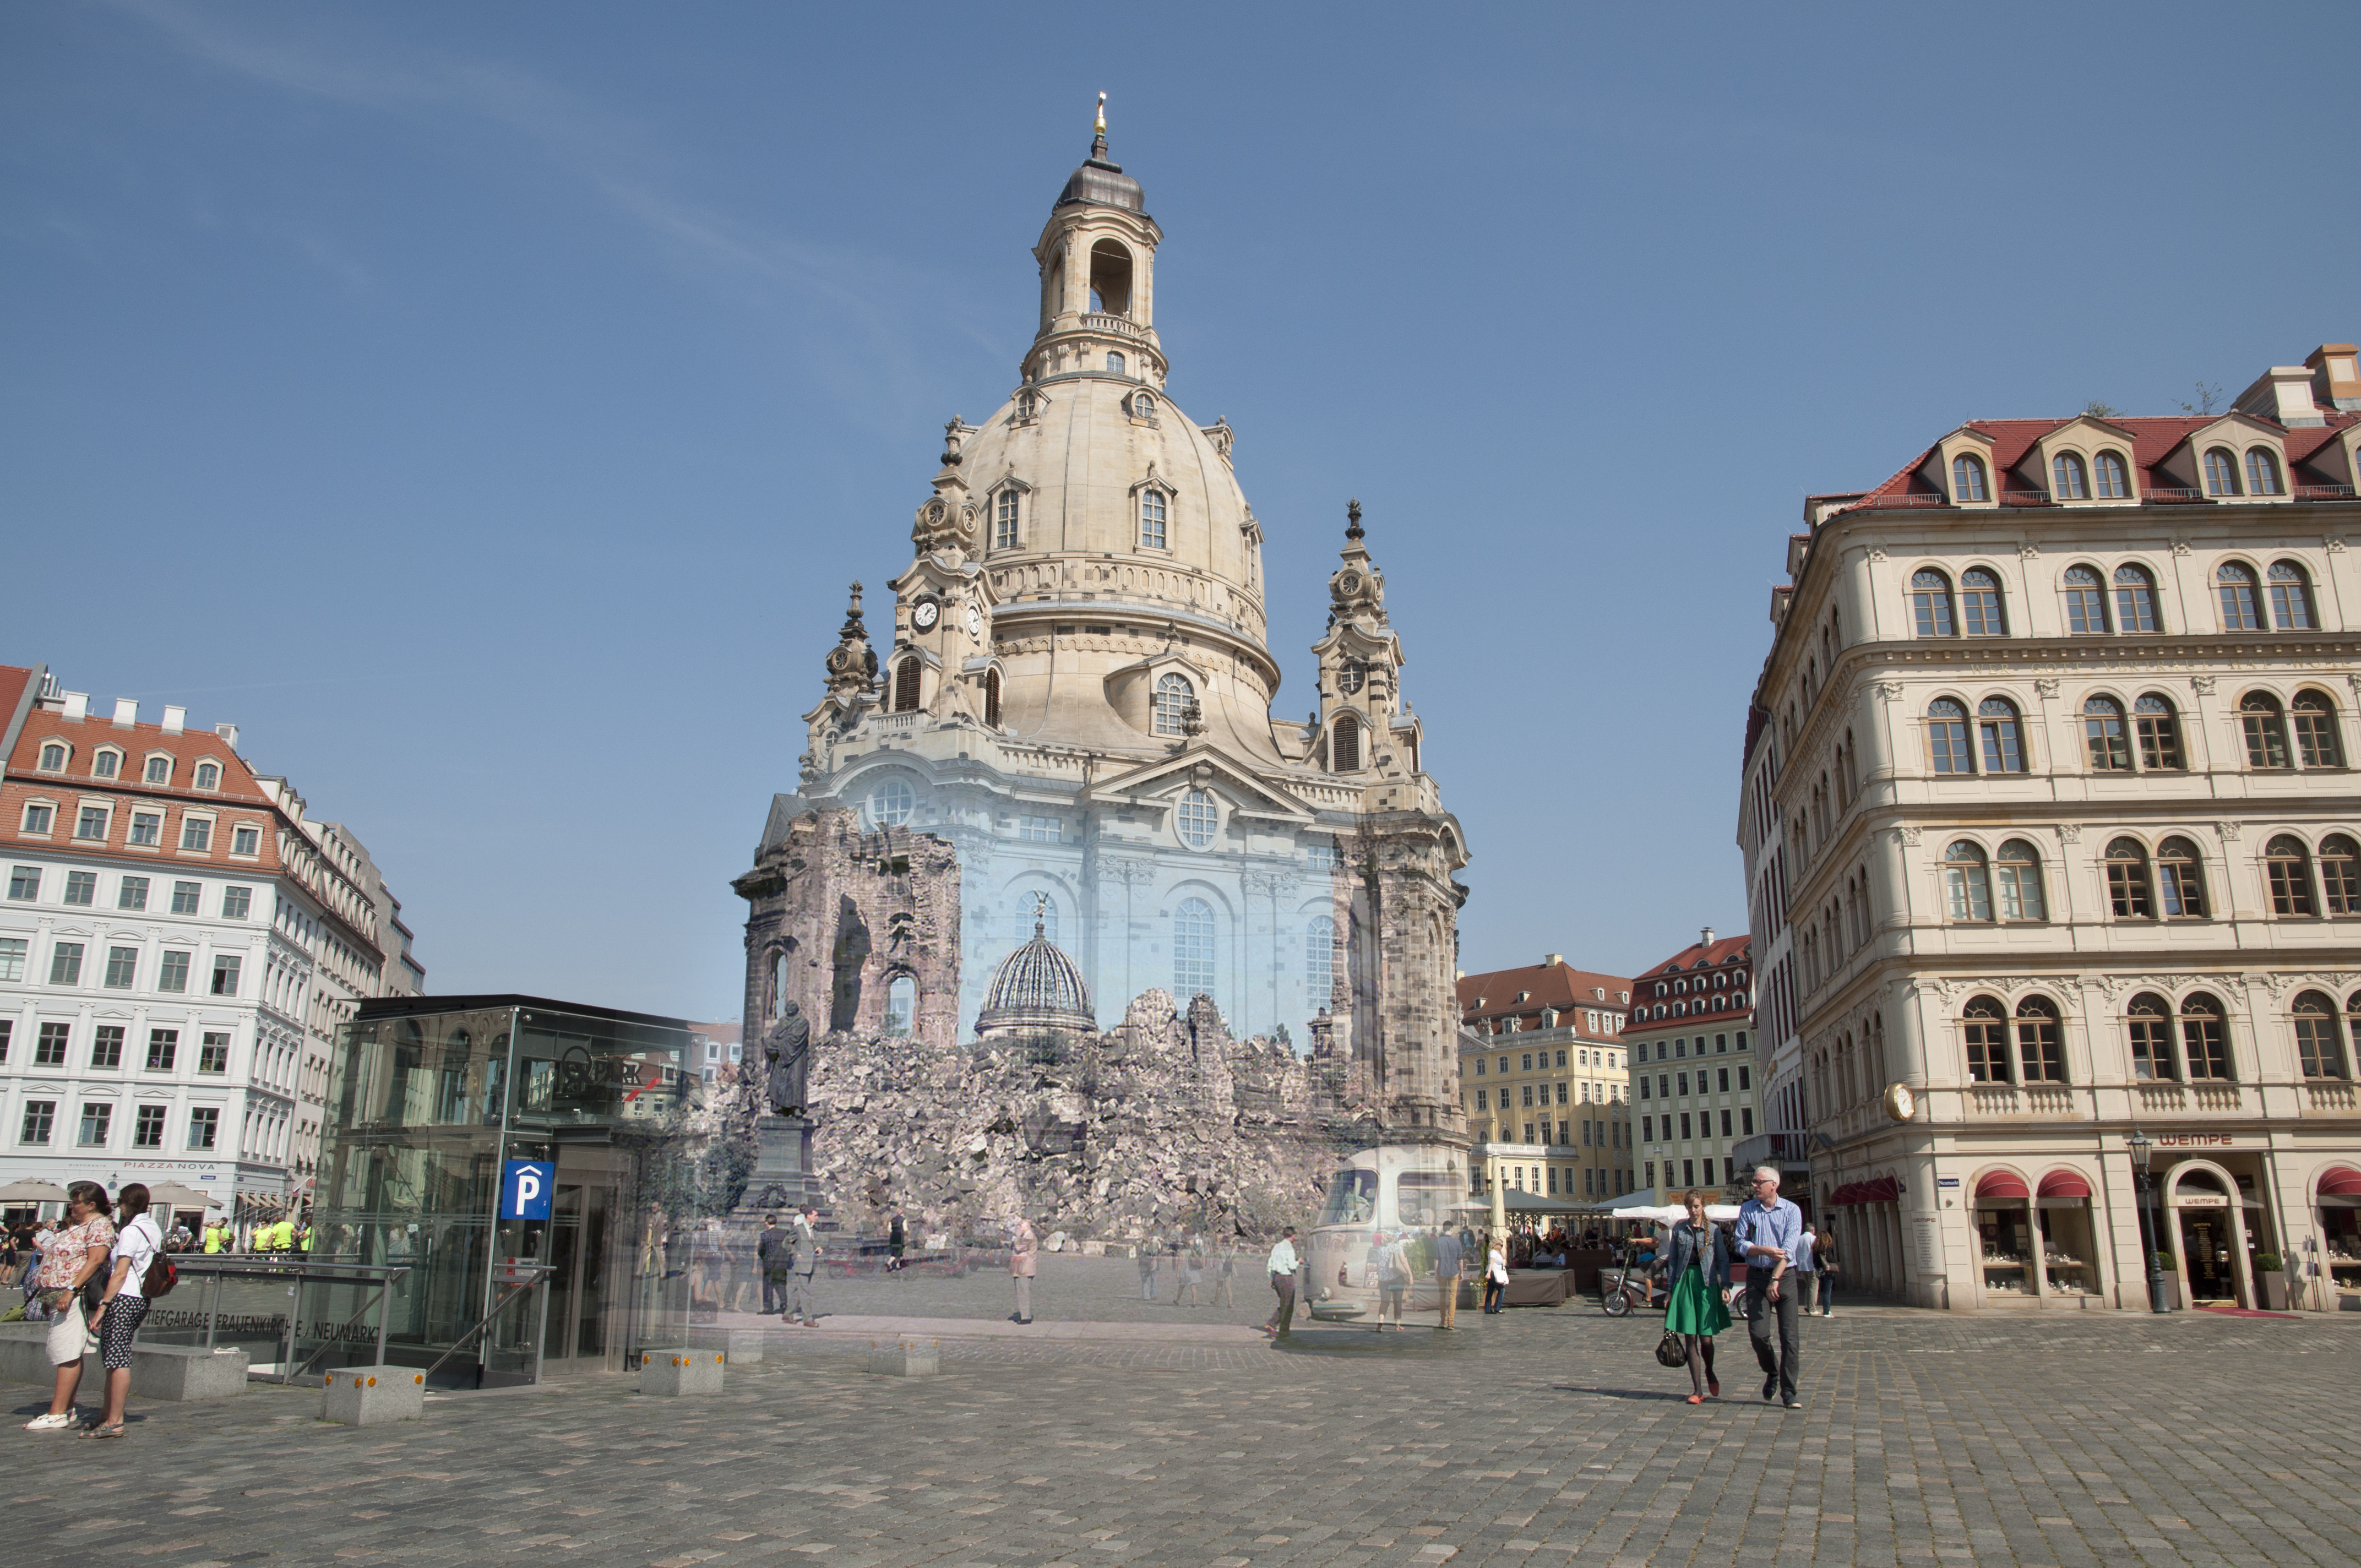
\includegraphics[width=\textwidth]{gfx/1950_2014_Frauenkirche.jpg}
   \caption{Frauenkirche in Dresden, destroyed during World War II,
   \textcopyright\ Sergey Larenkov, printed with permissio}
   \label{fig2}
\end{figure}

When done manually, the photographer must attempt to find the original viewpoint 
usually by visual inspection of the original image and trying to match the
current camera parameters --- camera position, camera rotation, focal length,
possibly principal point --- to the original.
The procedure is often carried out by placing the camera on a tripod and
comparing a printout of the original image with what can be seen through the
viewfinder or the camera screen. The number of parameters to match as well as
the difficulty to estimate them purely from comparing images makes the process
error-prone and tedious.

The advancement of mobile phones or tablet computers with integrated cameras and
larger screens
presents the opportunity to develop applications which can assist in this
endeavour, which is impossible on digital cameras due to their closed
infrastructure not permitting running user programs.

\end{document}
% ********************************************************************

